\begin{pycode}

\end{pycode}

\section{Séance 2 - Fréquence de résonance et fonction de transfert}


\subsection{Objectifs}
La première séance de ce projet a permis les observations suivantes :
\begin{itemize}
    \item La fréquence idéale du système se situe à 6.78 MHz (Figure \ref{fig: S}).
    \item À la fréquence de 2.6 MHz, la résistance étant constante en fonction de la position,
    il est difficile d'avoir un capteur de position avec ce système.
    \item Au-delà de la fréquence de 2.6 MHz, le modèle théorique devient trop différent de la réalité.
    \item À une fréquence proche de 150 kHz, pour l'inductance et la résistance, il est possible
    de considérer qu'entre deux positions, le système se comporte de manière linéaire.  
\end{itemize}

\vspace{0,2cm}

Le but de cette séance sera donc d'abaisser la fréquence de résonance du système à une valeur
exploitable. L'abaissement de la fréquence de résonance se fait par la mise en parallèle d'une 
capacité.

\begin{figure}[H]
    \centering
    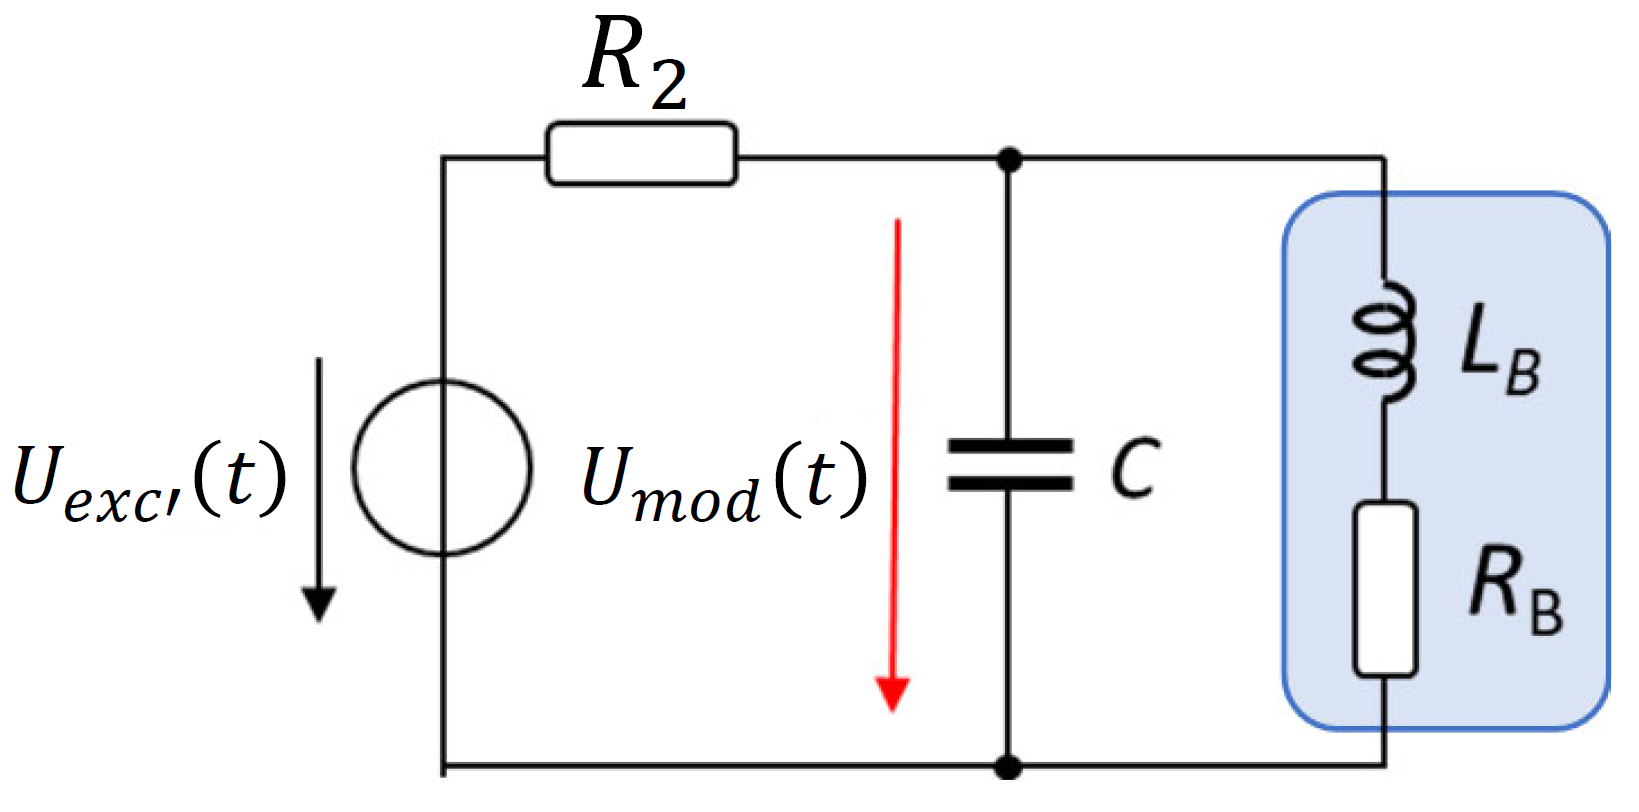
\includegraphics[width=10cm]{Images/Seance2/Circuit_resonant.png}
    \caption{Schéma du circuit résonant}
    \label{fig:circ_res}
\end{figure}
\vspace{0,2cm}

Cette capacité $C$ étant fournie, la fréquence de résonance sera déterminée théoriquement puis par
manipulation. Enfin, une résistance sera ajoutée pour obtenir une tension comme conditionneur pour le 
circuit résonnant. 



\subsection{Théorie}
\subsubsection{Signal d'excitation}
Le signal d'excitation est un signal carré, de fréquence $f$ et d'amplitude $A$. Par décomposition
en série de Fourrier, ce signal peut être exprimé comme suit :

\begin{equation*}
U_{exc}(t) = \frac{4}{\pi} A \cdot [\sin(\omega \cdot t)+\frac{1}{3}\sin(3\cdot\omega \cdot t)+\frac{1}{5}\sin(5\cdot\omega \cdot t)+...]     
\end{equation*}
\vspace{0,2cm}

Le signal $U_{exc}(t)$ est traité par un filtre passe-bande RLC, conservant uniquement la première
harmonique. Le signal d'excitation devient donc :

\begin{equation*}
    U_{exc'}(t) = \frac{4}{\pi} A \cdot \sin(\omega \cdot t)
\end{equation*}

Ce signal sera celui appliqué à la maquette.

\subsubsection{Fréquence de résonance}

La fréquence de résonance est donnée par l'équation suivante :

\begin{equation}
    f_0 = \frac{\omega_0}{2\pi} = \frac{1y}{2\pi}\sqrt{\frac{1}{L_B\cdot C}-\frac{R_B^2}{L_B^2}}
    \label{eq:freq_res}
\end{equation}

Avec $L_B$ l'inductance de la bobine, $R_B$ sa résistance et C la capacité de précision.
\vspace{0,2cm}

Lors du calcul, il est important de prendre en compte que $L_B$ et $R_B$ dépendent de la fréquence.
Cette équation est donc implicite et nécessite une itération et une interpolation des données pour
calculer la fréquence de résonance.


\subsubsection{Optimisation de la sensibilité}

Pour un circuit en parallèle, la sensibilité à la position de repos et à la fréquence de résonance
est maximisée lorsque $R_0$ est égale à $R_P$.

\begin{figure}[H]
    \centering
    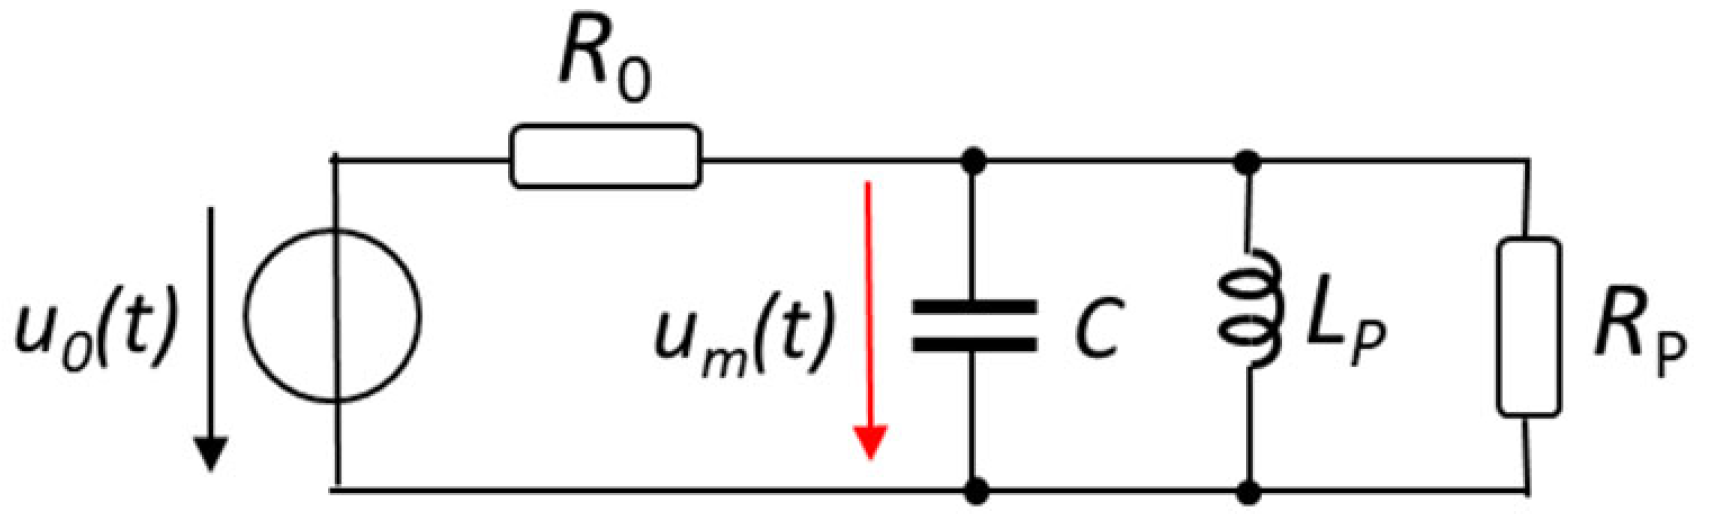
\includegraphics[width=10cm]{Images/Seance2/Circuit_para.png}
    \caption{Schéma du circuit résonant parallèle}
    \label{fig:circ_res_para}
\end{figure}

\vspace{0,2cm}

En effet, à la fréquence de résonance, la capacité et l'inductance peuvent être ignorées. Le système
se comporte alors comme un diviseur résistif.
\begin{figure}[H]
    \centering
    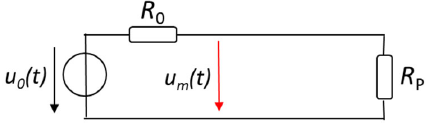
\includegraphics[width=10cm]{Images/Seance2/Circuit_ressss.png}
    \caption{Schéma du circuit résonant parallèle}
    \label{fig:circ_ressss}
\end{figure}

Il est donc possible d'écrire l'équation suivante :

\begin{equation*}
    U_m(t) = \frac{R_P}{R_0+R_P}U_0(t)
\end{equation*}
Pour notre système :
\begin{equation*}
    U_m(t) = \frac{R_P}{R_0+R_P}\cdot\frac{4}{\pi} A \cdot \sin(\omega \cdot t) 
\end{equation*}

Ce qui donne en valeur crête :

\begin{equation}
    U_m = \frac{R_P}{R_0+R_P}\cdot\frac{4}{\pi} A 
    \label{eq:crete}
\end{equation}

Le système utilisé ayant sa résistance et son inductance en série, il convient de les transformer en
parallèle. La conversion est régie par les équations suivantes :

\begin{equation*}
L_P = L_B \cdot (1+ \frac{1}{Q^2})
\end{equation*}
\begin{equation}
    R_P = R_B \cdot (1 + Q^2)
    \label{eq:res_equi}
\end{equation}
\begin{equation}
    Q = \frac{\omega_0\cdot L_B}{R_B}
    \label{eq:quali}
\end{equation}

\subsubsection{Fonction de transfert}
La fonction de transfert du système est donnée par l'équation suivante :
\begin{equation}
    \underbar{H}(\underbar{$Z_b$}) = \frac{\underbar{$Z_b$}}{(1+j\cdot\omega \cdot C \cdot R_0)\underbar{$Z_b$}+R_0}
    \label{eq:trsf}
\end{equation}

\subsection{Pratique}
\subsubsection{Montage}
\begin{figure}[H]
    \centering
    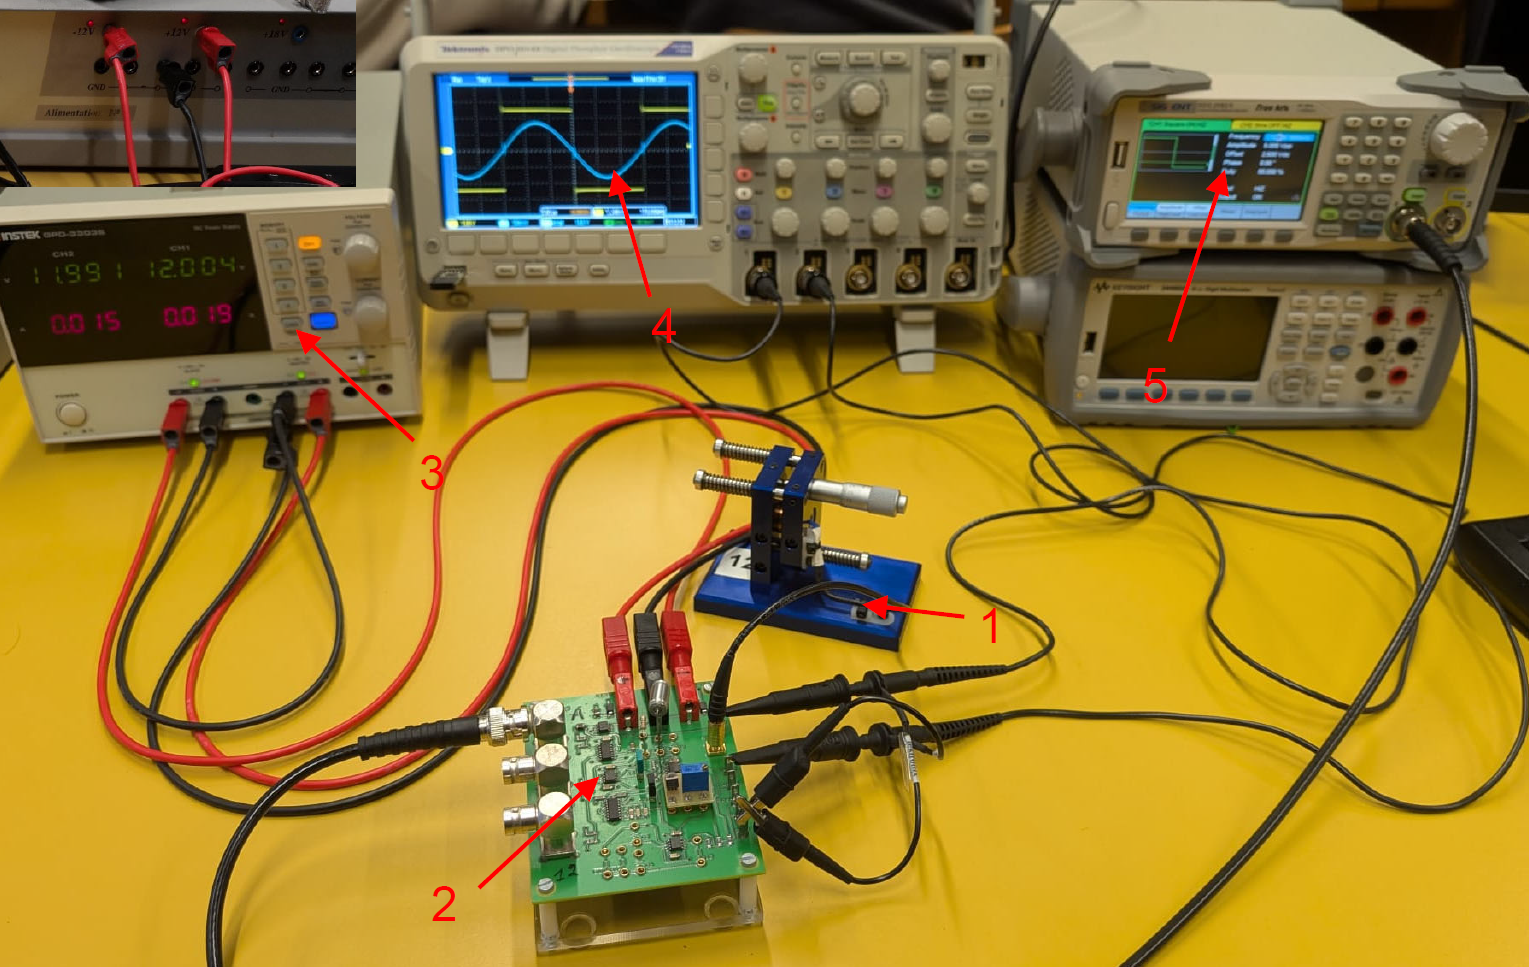
\includegraphics[width=15cm]{Images/Seance2/Montage.png}
    \caption{Montage}
    \label{fig:montage}
\end{figure}
\begin{enumerate}
    \item Maquette
    \item Carte électronique
    \item Alimentation
    \item Oscilloscope
    \item Générateur de signaux
\end{enumerate}

La sonde 1 est sur le signal d'excitation de la carte ($U_{exc}$), la sonde 2 est sur la sortie du
système ($U_{mod}$). La maquette est 


\subsubsection{Fréquence de résonance}
Pour rechercher la fréquence de résonance, la capacité de précision a été montée sur l'emplacement C2.
 La fréquence d'excitation a ensuite été ajustée jusqu'à ce que les deux tensions soient en phase. Les deux tensions sont en
phase lorsqu'elles passent à zéro au même moment.
\begin{figure}[H]
    \centering
    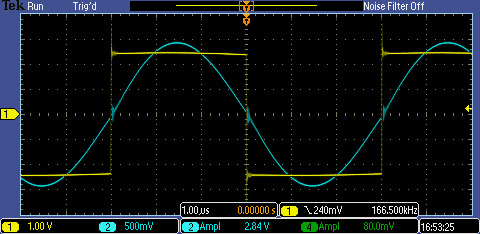
\includegraphics[width=10cm]{Images/Seance2/TEK00000.PNG}
    \caption{Recherche de la fréquence de résonance}
    \label{fig:freq_oscillo}
\end{figure}

Il est possible d'observer que la fréquence de résonance $f_0$ est de 166.5 kHz.
\vspace{0,2cm}

Après remplacement de la résistance $R_2$ par $R_0$, l'amplitude du signal de sortie $U_{mod}$ 
a été mesurée au multimètre pour une meilleure précision. Il est  important de noter que cet
appareil donne une valeur RMS de l'amplitude, il faudra donc multiplier par $\sqrt{2}$ la valeur
mesurée pour avoir la valeur crête de $U_{mod}$.

\subsection{Résultats}
\subsubsection{Fréquence de résonance}

Comme vu dans la partie pratique, la fréquence de résonance mesurée $f_0$ est de 166.5 kHz.

\vspace{0,2cm}

Le calcul théorique a été fait selon l'équation \ref{eq:freq_res}.
Comme précisé, les valeurs de l'inductance et de la résistance varient en fonction de la fréquence.
Le calcul a été réalisé itérativement, en effectuant une interpellation linéaire des caractéristiques
de la maquette, grâce au programme MatLab et a convergé vers une valeur de 168.1 kHz 

\begin{table}[H]
    \centering
    \begin{tabular}{|c|c|}
        \hline
    $f_0$    & $f_{0,th}$  \\ \hline
    166.5 kHz & 168.1 kHz \\ \hline
    \end{tabular}
    \caption{Résumé des fréquences de résonance}
    \label{tab:freq_res}
\end{table}

\subsubsection{Optimisation de la sensibilité}

Les calculs ont été effectués selon les équations \ref{eq:res_equi} et \ref{eq:quali}. Dans un premier
temps, le facteur de qualité à $f_{0,th}$ a été déterminé.

\begin{equation*}
    Q=13.29
\end{equation*}

Il a ensuite été possible de déterminer $R_P$.

\begin{equation*}
    R_P=322.66 \text{ }\Omega
\end{equation*}
La résistance réelle utilisée a été mesurée à 324 $\Omega$.
\vspace{0,2cm}

\begin{table}[H]
    \centering
    \begin{tabular}{|c|c|}
    \hline
    $R_P$     & $R_0$  \\ \hline
    322.66 $\Omega$ & 324 $\Omega$ \\ \hline
    \end{tabular}
    \caption{Résistance calculée et utilisée}
    \label{tab:Resi}
    \end{table}

La valeur crête théorique de $U_{mod}$ a été calculée grâce à l'équation \ref{eq:crete} :
\begin{equation*}
    U_{mod,th} = \frac{322.66}{324+322.66}\cdot\frac{4}{\pi}\cdot \frac{5}{2} = 1.588\text{ V}
\end{equation*} 
\vspace{0,2cm}
La valeur crête de la tension de sortie $U_{mod}$ a été mesurée comme précisé précédemment.
\begin{equation*}
    U_{mod,RMS} = 1.074{ V}
\end{equation*} 
\begin{equation*}
    U_{mod} = U_{mod,RMS}\sqrt{2} = 1.519{ V}
\end{equation*} 


\subsubsection{Fonction de transfert}
La fonction de transfert à la fréquence de résonance a été calculée selon l'équation \ref{eq:trsf}
pour les différentes positions.
\begin{figure}[H]
    \centering
    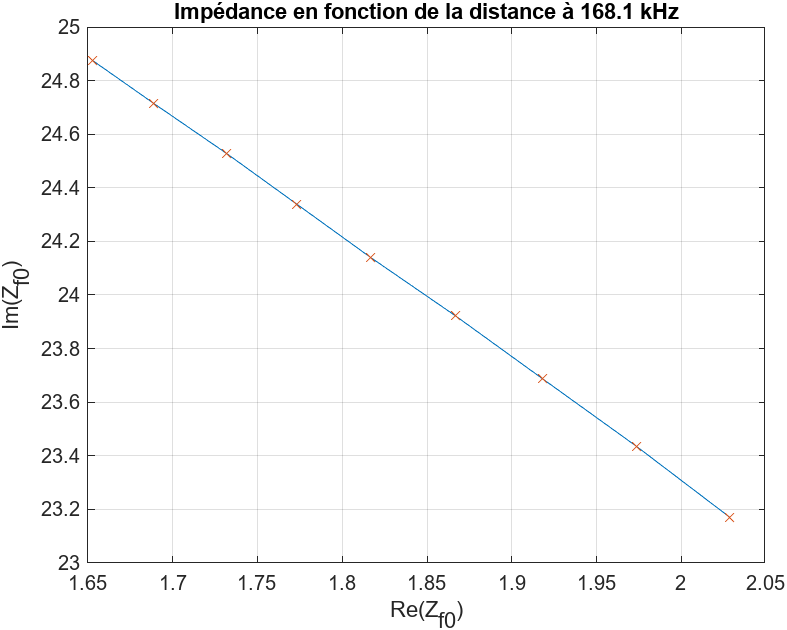
\includegraphics[width=15cm]{Images/Seance2/impedance_complexe_168.png}
    \caption{Représentation dans le plan complexe de l'impédance}
    \label{fig:impe}
\end{figure}

\begin{figure}[H]
    \centering
    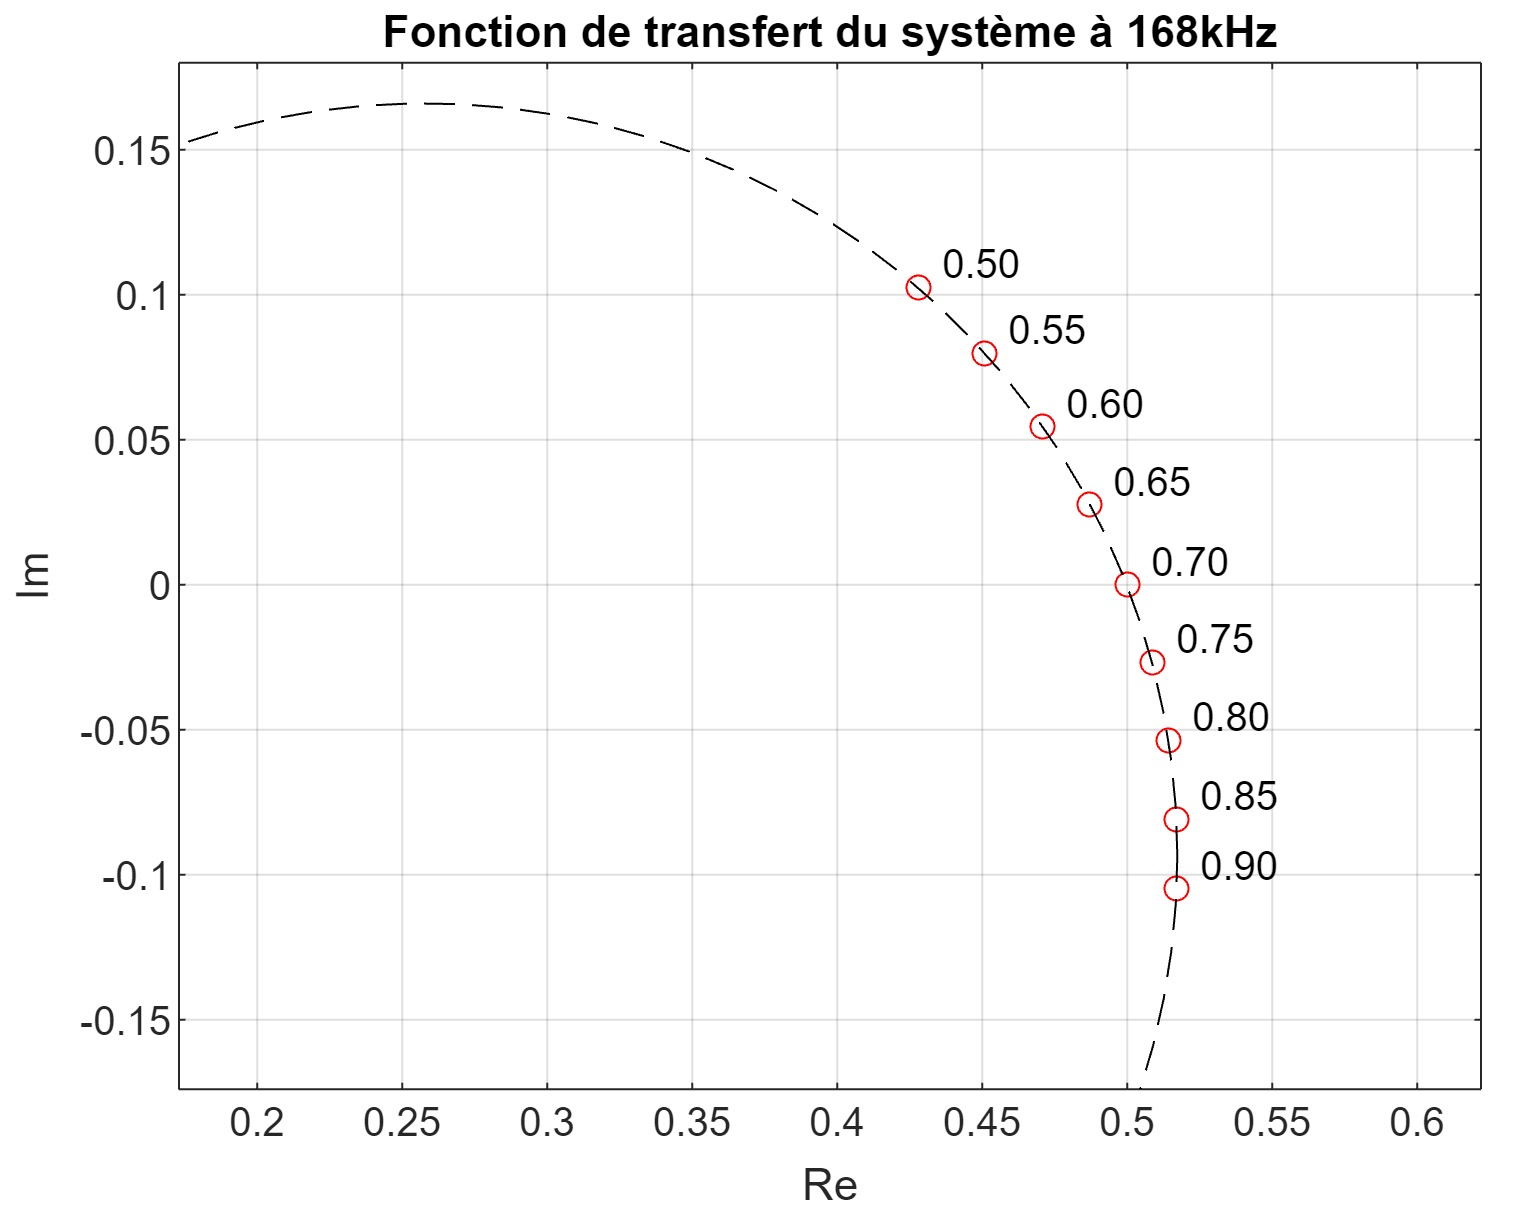
\includegraphics[width=15cm]{Images/Seance2/Transfert_mobius.jpg}
    \caption{Représentation dans le plan complexe de la fonction de transfert}
    \label{fig:transf}
\end{figure}

\subsection{Analyse}
En ce qui concerne la fréquence de résonance, la valeur calculée et celle trouvée par recherche sont
relativement proches, $\pm$ 1 \%. La différence peut venir de plusieurs sources. 
\vspace{0,2cm}

Dans un premier temps, l'erreur
peut venir des calculs. En effet, les données utilisées sont une interpolation des mesures. Il est
donc possible, quoique peu probable, qu'elles ne reflètent pas la réalité. 
\vspace{0,2cm}

Dans un second temps, il est possible que la recherche n'ait pas été effectuée correctement. Comme
il est possible de le deviner sur la figure \ref{fig:freq_oscillo}, le signal est bruité à 0 V. Il 
est donc possible qu'une légère erreur ait été commise.
\vspace{ 0,4cm}

Pour ce qui est de l'optimisation de la sensibilité, le seul point de contrôle disponible est la 
valeur crête de $U_{mod}$.

\begin{table}[H]
    \centering
    \begin{tabular}{|c|c|}
    \hline
    $U_{mod}$     & $U_{mod,th}$  \\ \hline
    1.519 V & 1.588 V \\ \hline
    \end{tabular}
    \caption{Tensions de sortie}
    \label{tab:Umod}
\end{table} 

Les deux valeurs ayant moins de 5\% de variation, il est cohérent de penser que la théorie est en 
adéquation avec la pratique. Il est donc censé d'estimer que la sensibilité est maximisée pour cette
fréquence. 

\vspace{ 0,4cm}
Enfin, la fonction de transfert montre une distribution circulaire sur le plan complexe. 
Cette distribution est attendue. De plus, la fonction de transfert est uniquement réel à la position
de repos, respectivement 0.7mm, ce qui est attendu. Il est donc fortement probable que les paramètres
choisis, respectivement la fréquence de résonance ainsi que la résistance soient corrects pour ce
système.

\subsection{Conclusion}

Durant cette séance, il a été possible de déterminer la fréquence de résonance du système.
Cette fréquence est de 166.5 kHz. La fréquence de résonance théorique varie légèrement, respectivement
de 1\%. 

\vspace{0.2cm}
Il a également été possible d'optimiser la sensibilité du système.
\vspace{0.2cm}

Enfin, la représentation de Möbius de la fonction de transfert a validé les point précédents, en
validant la position de repos à 0.7mm.